%
% $RCSfile: legacy_host.tex,v $
%
% Copyright (C) 2002-2008. Christian Heller.
%
% Permission is granted to copy, distribute and/or modify this document
% under the terms of the GNU Free Documentation License, Version 1.1 or
% any later version published by the Free Software Foundation; with no
% Invariant Sections, with no Front-Cover Texts and with no Back-Cover
% Texts. A copy of the license is included in the section entitled
% "GNU Free Documentation License".
%
% http://www.cybop.net
% - Cybernetics Oriented Programming -
%
% http://www.resmedicinae.org
% - Information in Medicine -
%
% Version: $Revision: 1.1 $ $Date: 2008-08-19 20:41:07 $ $Author: christian $
% Authors: Christian Heller <christian.heller@tuxtax.de>
%

\section{Legacy Host}
\label{legacy_host_heading}
\index{Legacy Host}
\index{Legacy Systems}
\index{Host}
\index{Mainframe}
\index{Common Business Oriented Language}
\index{COBOL}
\index{Programming Language One}
\index{PL/I}
\index{Virtual Storage Access Method}
\index{VSAM}
\index{Third Party Maintenance}
\index{TPM}
\index{Customer Information Control System}
\index{CICS}

Finally, there is often a need to integrate \emph{Legacy Systems}, which are a
special variant of remote software systems running on computers with an older
architecture. Those computers are also named \emph{Host}, as in the example of
figure \ref{legacy_figure}, or \emph{Mainframe}. The applications running on
them are programmed in languages like the \emph{Common Business Oriented Language}
(COBOL) or \emph{Programming Language One} (PL/I) \cite{pli}, the latter
developed as an \emph{International Business Machines} (IBM) \cite{ibm} product
in the mid 1960's.

\begin{figure}[ht]
    \begin{center}
        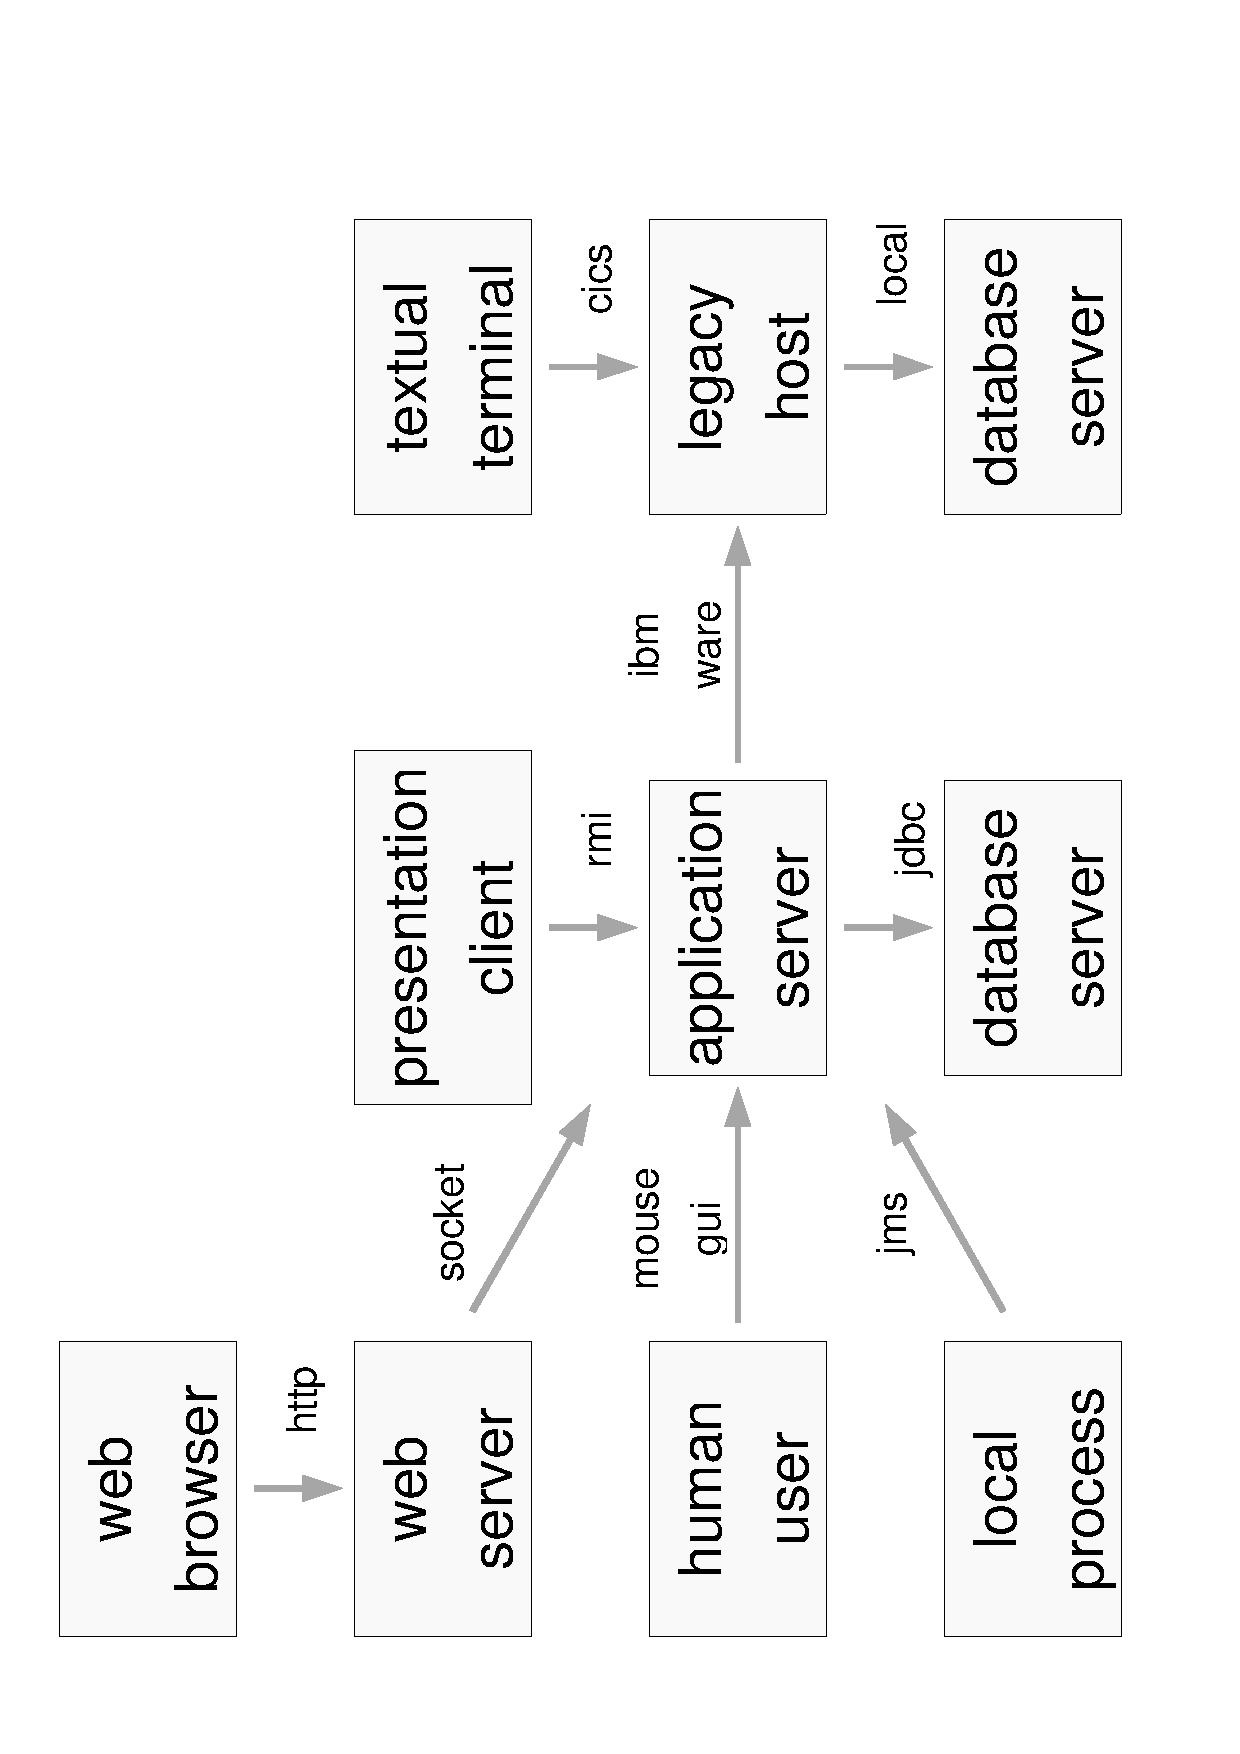
\includegraphics[scale=0.3,angle=-90]{graphic/legacy.pdf}
        \caption{Legacy Host}
        \label{legacy_figure}
    \end{center}
\end{figure}

Host computers manage nearly everything an ancient information technology
environment needs. They are responsible for persistence and processing of data.
Often, they contain hierarchical databases \cite{oolegacysystems} using flat
files like the \emph{Virtual Storage Access Method} (VSAM) format. True clients
do not exist here. Character-based terminals are the way to communicate with
the host which controls all interaction (including keyboard and screen), within
a \emph{Third Party Maintenance} (TPM) \emph{Customer Information Control System}
(CICS) runtime environment.
